\documentclass[conference]{IEEEtran}
\IEEEoverridecommandlockouts
\usepackage{cite}
\usepackage{amsmath,amssymb,amsfonts}
\usepackage{algorithmic}
\usepackage{graphicx}
\usepackage{textcomp}
\usepackage{xcolor}
\def\BibTeX{{\rm B\kern-.05em{\sc i\kern-.025em b}\kern-.08em
    T\kern-.1667em\lower.7ex\hbox{E}\kern-.125emX}}

\usepackage{listings}

\lstset{
	numbers=left,
	stepnumber=1,
	firstnumber=1,
	numberstyle=\scriptsize,
	extendedchars=true,
	breaklines=true,
	frame=single,
	showstringspaces=false,
  aboveskip=1.5em,
	xleftmargin=2.5em,
	framexleftmargin=2em,
	basicstyle=\scriptsize,
}

\renewcommand{\lstlistingname}{Código}
\renewcommand{\lstlistlistingname}{Lista de Códigos}


\begin{document}

\title{Classificação de \textit{issues} do Github relacionadas a Segurança}

\author{\IEEEauthorblockN{1\textsuperscript{st} Bruno Gonçalves de Oliveira}
    \IEEEauthorblockA{
        \textit{Universidade Federal do Paraná (UFPR)}\\
        Curitiba– PR – Brasil \\
        bruno.mphx2@gmail.com}
    \and
    \IEEEauthorblockN{2\textsuperscript{nd} Diogo Cezar Teixeira Batista}
    \IEEEauthorblockA{
        \textit{Universidade Federal do Paraná (UFPR)}\\
        Curitiba– PR – Brasil \\
        diogocezar@utfpr.br}
}

\maketitle

\begin{abstract}
    As \textit{issues} do GitHub representam grande parte da evolução dos projetos \textit{OpenSource}. Este trabalho propõe uma solução para classificar \textit{issues} que podem ou não estar relacionadas a segurança da informação. As mensagens serão analisadas utilizando as palavras frequentes em textos referentes a segurança. Utiliza-se a técnica de \textit{Bag-of-Words} em conjunto com \textit{TF-IDF} para a criação do \textit{dataset} de representação. Na sequência, experimentos com  classificadores foram realizados para explorar qual a melhor ténica a ser adodata para o problema em questão. Os melhores resultados apresentam uma acurácia superior a 80\%, o que demonstra que as soluções exploradas são plausíveis e podem ser melhoradas como é explorado na seção de trabalho futuros.
\end{abstract}

\begin{IEEEkeywords}
    Issues, GitHub, Segurança da Informação, Classificadores, Aprendizagem de Máquina
\end{IEEEkeywords}

\section{Introdução}

O controle, gerenciamento e manutenção de arquivos, especialmente no âmbito do desenvolvimento de \textit{software}, sempre foi um desafio. Problemas recorrentes como: \textit{backups} não realizados, sobrescrita de arquivos ou dificil manutenabilidade de projetos desenvolvidos em equipes, são algumas das motivações para a utilização de algum sistema de versionamento de arquivos. \cite{Scott:ProGit}

Dentre as várias ferramentas existenstes no mercado, tais como: \textit{CVS}, \textit{Subversion}, \textit{TFS}, \textit{Mercurial}, o \textit{Git} se destaca por ter sido amplamente utilizado pela comunidade de desenvolvimento, com o advento da popularização dos projetos \textit{Open Source}. Tais projetos se consolidaram em ferramentas como o \textit{GitHub} que é uma plataforma para versionamento, gerenciamento e colaboração de projetos, que utiliza o \textit{Git} como base. \cite{Scott:ProGit}

São várias as possibilidades que essas ferramentas proporcionam para verionamento dos projetos, no \textit{GitHub}, por exemplo, existe uma sessão de \textit{issues} (problemas) na qual, os colaboradores de um projeto \textit{Open Source} podem cadastrar possíveis \textit{bugs}, melhorias, ou novas \textit{features} para os projetos.

Na descrição dessas \textit{issues}, feita através do preenchimento de um campo de texto, é possível identificar qual é o contexto em que se aplica determinada correção, melhoria ou \textit{feature}.

Eventualmente, dentre as correções realizadas nestes projetos, são identificados ajustes relacionados a segurança. Estas \textit{issues}, quando consideradas críticas, podem ser analisadas por outros especialistas para uma arguição mais detalhada e um possível aprimoramento.

Mas como identificar quais são os ajustes de um projeto que estão relacionados com segurança? Como separar estes ajustes para que especialistas possam analisar os cógidos? Essas perguntas guiam a motivação para o desenvolvimento deste trabalho.

Propõe-se a criação de uma ferramenta que utilize técnicas de aprendizagem de máquina para o desenvolvimento de um oráculo classificador que consiga analisar as palavras contidas nas mensagens das \textit{issues} de um dado projeto, e classificar se esta \textit{issue} está ou não relacionada no contexto de segurança da informação.

Por fim, discute-se os resultados obtidos dos experimentos e possíveis trabalhos futuros.

\section{Obtenção dos Dados}

Projetos \textit{Open Source} são, por essência, públicos na Internet, e por este motivo, suas \textit{issues} também estão dispostas de forma pública. A análise dessas mensagens faz parte da evolução dos projetos, nos quais os colaboradores podem entender os problemas, sugerir, implementar e finalizar os problemas encontrados.

A Figura \ref{fig:issues_example} mostra um exemplo de algumas issues do projeto Vue.js.

\begin{figure}[htbp]
    \centerline{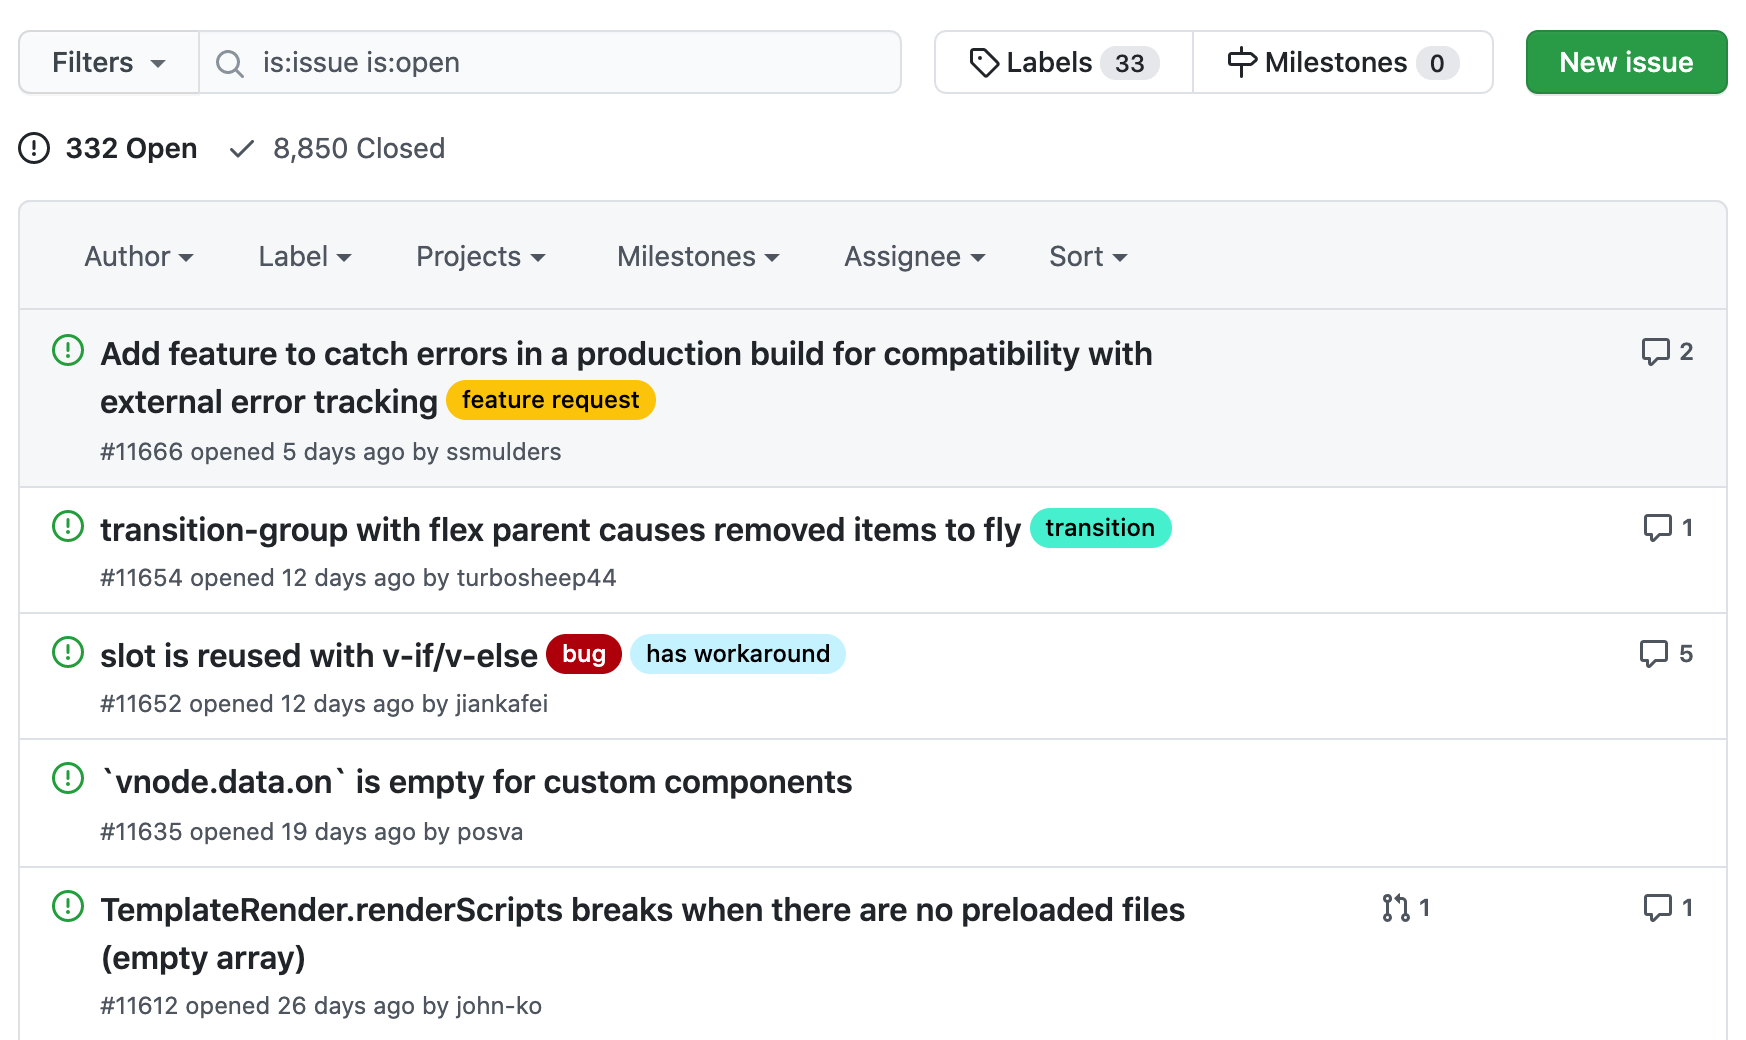
\includegraphics[width=25em]{images/issues_example.png}}
    \caption{Exemplos de Issues do Projeto Vue.js}
    \label{fig:issues_example}
\end{figure}

Para a extração dos dados das \textit{issues}, tanto para a base de treinamento quanto de para a base de testes, utilizou-se a a ferramenta \textit{github-csv-tools\footnote{https://github.com/gavinr/github-csv-tools}} que possibilita a exportação dos dados de um repositório do \textit{GitHub}, salvando as informações em um arquivo no formato CSV.

Os dados foram refinados para compor um arquivo CSV com 2 colunas. A primeira  indica se a \textit{issue} é um tópico relacionado a segurança ou não, e a segunda coluna representa de fato o texto coletado.

Um exemplo abreviado de cada classe pode ser vista no Código \ref{code:csv_example}.

\begin{lstlisting}[caption={CSV Exemplo com Base de Dados},captionpos=b,frame=single,label={code:csv_example}]
security,PushObserver can be used to push serverinitiated HTTP/2 requests into an OkResponseCache...
not,Handle LOCKED in conversions.Motivation...
\end{lstlisting}

Para a geração da base de testes, foram extraídas as \textit{issues} do projeto \textit{Wildfly\footnote{https://github.com/wildfly/wildfly}}. Já para a base de treinamento utilizou-se \textit{issues} dos projetos: \textit{https://github.com/square/okhttp/}, \textit{https://github.com/eclipse/jgit} e \textit{https://github.com/couchbase}.

Os dados de treinamento possuem \textbf{199} entradas, enquanto que para a base de teste foram utilizadas \textbf{211} entradas.

\section{Pré-processamento}

Após a obtenção dos dados, é importante a realização de algumas etapas de pré-processamento do texto, estes tratamentos procuram maximizar a representatividade das \textit{issues} de acordo com o seu significado.

Para isso, é necessário remover palavras que não representam o contexto das frases. Com esse objetivo, aplica-se técnicas de sanitização para a base de treinamento e testes.

As regras aplicadas foram:

\begin{enumerate}
    \item Transformar todo texto em minúsculo;
    \item Ignorar pontuações;
    \item Corrigir palavras com ortografia incorreta;
    \item Remover as chamadas \textit{stop words} que não acrescentam informação aos textos, por exemplo: \textit{of, a, in, on}.
\end{enumerate}

\section{Extração de Características}

Para a extração de características das bases de dados, utiliza-se uma técnica conhecida como \textit{Bag-of-Words} \cite{Mohey:Bag}. Nesta técnica, as sentenças são representadas através da identificação de suas palavras e a quantidade em que aparecem no texto. Por exemplo, considerando o seguinte texto, escrito por \textit{Charles Dickens}:

\begin{quote}
    It was the best of times,\\
    It was the wost of times,\\
    It was the age of wisdom,\\
    It was the age of follishness.
\end{quote}

Considerando palavras únicas, neste caso, teríamos um vocabulário com 10 palavras: [it, was, the, best, of, times, worst, age, wisdom, foolishness]

Na sequência deve-se criar os vetores que representam a quantidade de aparições de uma palavra no texto. Por exemplo, no documento ``It was the age of wisdom'' pode-se representar através de um vetor dado por: $[1, 1, 1, 0, 1, 0, 0, 1, 1, 0]$. Se novas frases, com palavras fora do vocabulário definido forem adicionadas, então essas serão descartadas.

Com os vetores de palavras formados com a identificação e a quantidade, é possível aplicar a técnica de \textit{TF-IDF (term frequency-inverce document frequency)}.  Nesta abordagem, valoriza-se o quão importante uma palavra é ao documento. O valor de \textit{TF-IDF} aumenta proporcionalmente conforme o número de vezes a palavra aparece no texto e é compensado pelo número de textos na base de dados, ajustando o número da frequência das palavras. \cite{Manning:InformationRetrieval}

Basicamente para cada uma das \textit{issues} já sanitizadas aplica-se uma contagem das palavras mais relevantes para o problema em questão. Essas palavras foram obtidas a partir de uma contagem das palavras que mais apareciam nas \textit{issues} que eram relacionadas à segurança.

Obteve-se as seguintes palavras: ['security', 'secure', 'vulnerable', 'leak', 'exception', 'crash', 'malicious',
'sensitive', 'user', 'authentication', 'protect', 'vulnerability', 'authenticator', 'auth', 'npe']

Após a aplicação destas técnicas, obtém-se 4 vetores que serão utilizados nas próximas fases do experimento. São eles: (x\_train, y\_train, x\_test, y\_test)

\section{Orquestrador dos Exerimentos}

Essencialmente em problemas que podem envolver diferentes classificadores, é bastante comum a realização dos experimentos em diferentes abordagens, utilizando classificadores diferentes, e para cada um dos classificadores, parâmetros diferentes.

Com o intúito de automatizar o processo de variação entre os experimentos, desenvolveu-se um sistmea orquestrador de classificadores.

Este sistema utiliza um arquivo no forma \textit{JSON} para definir 2 principais blocos: configurações e experimentos.

No bloco de configurações, é possível definir quais serão os arquivos de entrada e saída para a realização dos experimentos. Já no bloco de experimentos define-se um \textit{array} com todos os experimentos a serem realizados.

Um exemplo do arquivo de orquestração pode ser visto no Código \ref{code:orquestrador}.

\begin{lstlisting}[caption={JSON do Orquestrador},captionpos=b,frame=single,label={code:orquestrador}]
{
    "configs": {
        "train": "data/train.csv",
        "test": "data/test.csv",
    },
    "experiments": [
        {
        "classifier": "logistic_regression",
        "parameters": {"solver": "lbfgs"}
        },
        {
        "classifier": "knn",
        "parameters": {"n_neighbors": 7}
        },
        ...
    ]
}
\end{lstlisting}

Para cada uma das ocorrências no vetor de experimentos, o programa desenvolvido utiliza implementações do \textit{framework} \textit{\footnote{https://scikit-learn.org/}scikit-learn} para o treinamento do classificador. Utlizando como fonte de dados, as entradas já tratados anteriormente (x\_train, y\_train, x\_test, y\_test). Os resultados são armazenados automaticamente em um arquivo no formato CSV que tabula os resultados obtidos em cada um dos experimentos. Os campos salvos são: \textit{Classifier, F1Score, Accuracy e Time (s)}. Além disso, para cada execução são armazenadas as matrizes de confusão como imagens e também como arquivos CSV.

\section{Classificação}

Para o trabalho foram utilizados 8 classificadores:

\begin{itemize}
    \item \textit{Linear Discriminant Analysis} (LDA): técnica de transformação linear que maximiza a característica que se pode separar entre classes e minimiza o espalhamento dentro da classe; \cite{Andrew:Statistical}
    \item Máquina de Vetores de Suporte \textit{Support Vector Machine} (SVM): o classificador tem como objetivo encontrar um hiperplano que maximiza a separabilidade das classes; \cite{Andrew:Statistical}
    \item Vizinhos mais próximos (\textit{KNN}): algoritmo utilizado para classificação que define a classe de uma nova amostra com base na representatividade de um conjunto de $k$ vizinhos mais próximos; \cite{Duda:Pattern}
    \item \textit{Multi-layer Perceptron} (MLP): é uma rede neural com múltiplas camadas compostas de neurônios que realizam o mapeamento das entradas ponderadas em um espaço não linear; \cite{Andrew:Statistical}
    \item O \textit{Perceptron} é um tipo de rede neural artificial que representa um classificador binário que mapeia sua entrada $x$ (um vetor de valor real) para um valor de saída $f(x)$ utilizando pesos para aprender ao logo do tempo; \cite{Rosenblatt1958ThePA}
    \item Uma árvore de decisão (\textit{Decision Tree}) consiste em uma coleção de nós internos e nós folhas, organizados em um modelo hierárquico como uma estrutura de dados, que orienta a classificação (baseado em comparações) de uma amostra a ser classificada. \cite{Duda:Pattern}
    \item O \textit{Multilayer Perceptron} (MLP) é semelhante ao \textit{Perceptron}, porém com a utilização de mais de uma camada para a aprendizagem ao longo do tempo;
    \item A técnica de mistura de gaussianas é uma abordagem probabilística para realizar um agrupamento do tipo \textit{soft clustering}. Este tipo de abordagem atribui um exemplo a uma classe com uma dada probabilidade; \cite{Pinkus99approximationtheory}
\end{itemize}

O orquestrador dos experimentos foi configurado para executar os experimentos com os classificadores: \textit{svm.LinearSVC}, \textit{KNeighborsClassifier}, \textit{GaussianNB}, \textit{LinearDiscriminantAnalysis}, \textit{LogisticRegression}, \textit{Perceptron}, \textit{DecisionTreeClassifier} e \textit{MLPClassifier}.

Os parâmetros utilizados foram os default em cada um dos classificadores. Com a exeção do \textit{KNeighborsClassifier} em que se testou com \textit{n\_neighbors: 7} e \textit{LogisticRegression} que se utilizou \textit{solver: lbfgs}.

\section{Resultados Obtidos}

Esta seção mostra os resultados obtidos após a execução do orquestrador para os diferentes classificadores.

\subsection{Avaliação de Desempenho}

Para a medição dos resultados utilizou-se a Acurácia e F1Score.

A Acurácia mede a razão entre o número de previsões corretas e o número total de amostras de entrada e é dada por:

\begin{equation}
    \text{Acurácia}=\frac{\text{VP} + \text{VN}}{\text{VP} + \text{VN} + \text{FP} + \text{FN}}
\end{equation}

onde, $VP$ é os positivos verdadeiros e $FN$ os negativos falsos.

Já a métrica de F1Score, é dada por:

\begin{equation}
    \text{F1Score} = 2 \cdot \frac{P\cdot R}{P + R}
\end{equation}

onde $P$ (precisão) é o número de verdadeiros positivos divido pelo número de positivos estimados pelo modelo. e $R$ (\textit{recall}) é o número de verdadeiros positivos divido pela somade $VP + FN$.

Os resultados obtidos estão dispostos na Tabela \ref{tab:resultados_experimentos}.

\begin{table}[!htb]
    \centering
    \begin{tabular}{|c|c|c|c|}
        \hline
        \textbf{Classifier}        & \textbf{Accuracy} & \textbf{F1Score} & \textbf{Time (s)} \\ \hline
        LinearDiscriminantAnalysis & 0.867             & 0.865            & 0.183             \\ \hline
        LogisticRegression         & 0.867             & 0.865            & 0.191             \\ \hline
        DecisionTreeClassifier     & 0.867             & 0.865            & 0.193             \\ \hline
        MLPClassifier              & 0.867             & 0.865            & 0.302             \\ \hline
        svm.LinearSVC              & 0.867             & 0.865            & 1.903             \\ \hline
        Perceptron                 & 0.862             & 0.861            & 0.17              \\ \hline
        KNeighborsClassifier       & 0.533             & 0.696            & 0.229             \\ \hline
        GaussianNB                 & 0.471             & 0.307            & 0.192             \\ \hline
    \end{tabular}
    \vspace{0.2cm}
    \caption{Resultados dos Experimentos}
    \label{tab:resultados_experimentos}
\end{table}

As matrizes de confusão dos classificadores: \textit{DecisionTreeClassifier}, \textit{GaussianNB} \textit{KNeighborsClassifier} e \textit{LinearDiscriminantAnalysis} estão dispostas na Figura \ref{fig:conf_mat_1}. Já para os classificadores: \textit{svm.LinearSVC}, \textit{LogisticRegression}, \textit{MLPClassifier} e \textit{Perceptron} as representações estão dispostas na Figura \ref{fig:conf_mat_2}.

\begin{figure}[htbp]
    \centerline{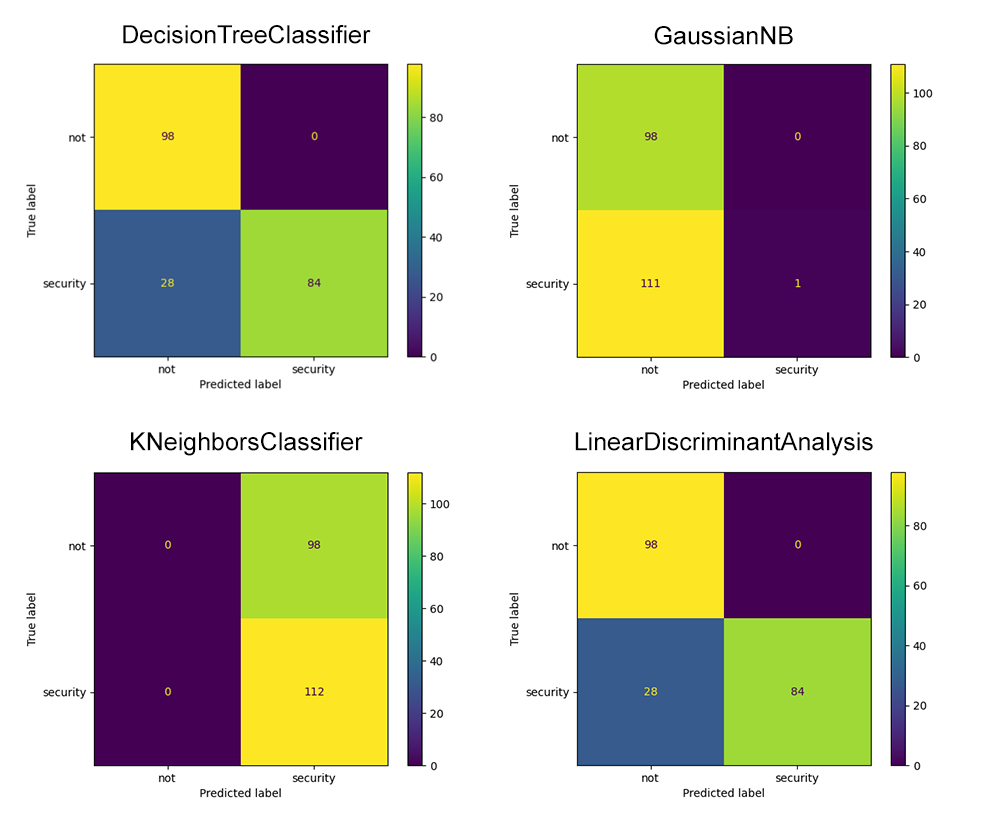
\includegraphics[width=25em]{images/conf_mat_1.png}}
    \caption{Matrizes de Confusão 1}
    \label{fig:conf_mat_1}
\end{figure}

\begin{figure}[htbp]
    \centerline{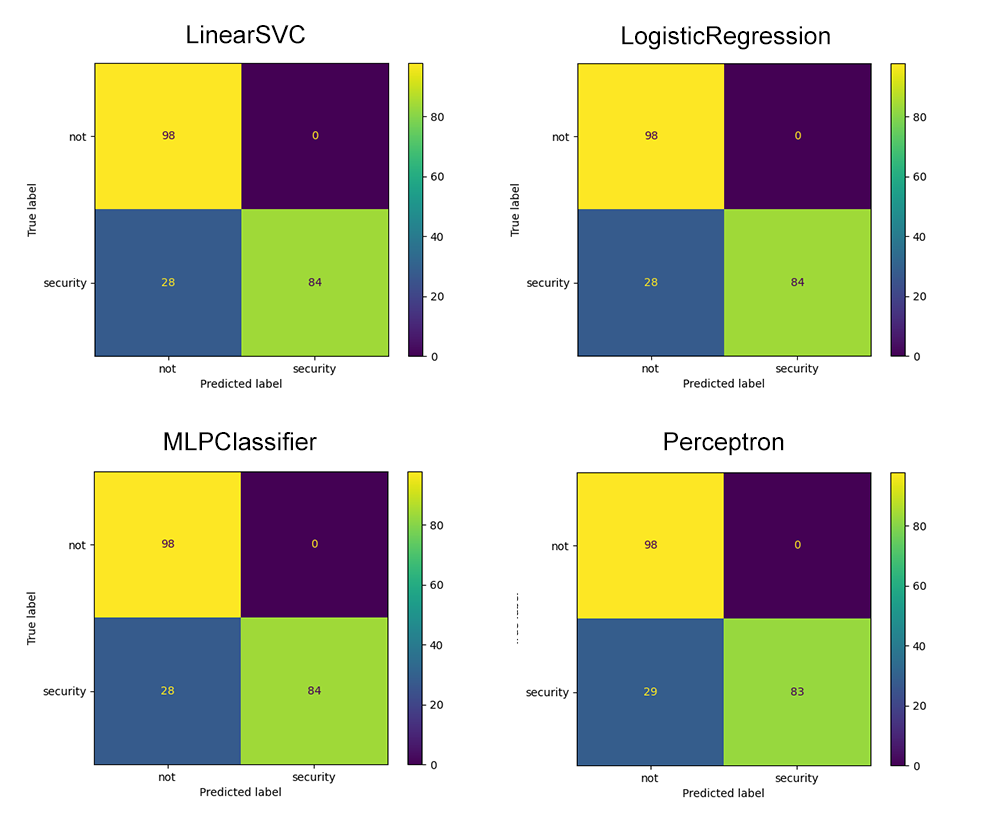
\includegraphics[width=25em]{images/conf_mat_2.png}}
    \caption{Matrizes de Confusão 2}
    \label{fig:conf_mat_2}
\end{figure}

\section{Conclusão}

Como é possível observar na Tabela \ref{tab:resultados_experimentos} os classificadores que utilizaram os algorítmos: \textit{LinearDiscriminantAnalysis}, \textit{LogisticRegression}, \textit{DecisionTreeClassifier}, \textit{MLPClassifier}, \textit{svm.LinearSVC} e \textit{Perceptron} tiveram resultados bastante semelhantes, com uma taxa de acurácia em torno de $0.86$ e um f1score também por volta de $0.86$. A duração do processo de classificação (anotada pela coluna Time (s)) demostram que para o volume de dados utilizado todos tem um tempo de treinamento bem baixo, retornando o resultado em menos de 2 segundos no pior caso.

Para o classificador \textit{KNeighborsClassifier} obteve-se um resultado bastante insatisfatório, com acurácia de $0.53$ e f1score de $0.69$. Isso se deve, pois os exemplos provavelmente foram projetados de forma esparça.

Já para o classificador \textit{GaussianNB} também obteve-se um resultado bastante insatisfatório, com acurácia de $0.47$ e f1score de $0.3$, e isso se deve também pela projeção esparçada dos exemplos.

Ainda nas matrizes da Figura \ref{fig:conf_mat_1}, nota-se que para os piores classificadores (neste problema) \textit{KNeighborsClassifier} e \textit{GaussianNB} houveram vários erros que praticamente anulam a eficiência do classificador.

Com relação às matrizes da Figura \ref{fig:conf_mat_2} é possível notar que praticamente o mesmo número de erros foi encontrado, muito provavelmente nos mesmo exemplos.

\section{Trabalhos Futuros}

A grande dificuldade encontrada no projeto foi a obtenção de uma base de dados rotulada. Toda a base utilizada foi tratada de forma manual. O que dificultou bastante a geração da base de testes e validação.

Para aumentar a base de treinamento de uma forma automatizada, propõe-se no futuro o desenvolvimento de um programa capaz de extrair automaticamente informações de \textit{issues} de repositórios do \textit{GitHub} marcados com um \textit{label} que contenha palavras relacionadas à segurança. O \textit{GitHub}, oferece uma API que possibilita a extração de informações dos projetos no formato JSON, o que facilitaria este processo. É possível notar que em alguns projetos, existem \textit{issues} pré-classificadas com \textit{labels}, como é o exemplo do repositório do projeto Angular, disponível em: https://github.com/angular/angular/labels?q=sec.

Outra estratégia poderia ser a aplicação de técnicas de \textit{Data Augmentation} para possibilitar a criação de características de forma sintéticas, refinando ainda mais os classificadores testados.

\section{Código Fonte}

O código fonte dos experimentos pode ser acessado em: https://github.com/bmphx2/aprendizagem-de-maquina

\bibliographystyle{IEEEtran}
\bibliography{IEEEabrv,IEEEexample.bib}

\end{document}